%Template criado para o PPGCC - UFOP
%e adaptado para DECOM - UFOP
%Baseado no template da COPPE - UFRJ
%Modificado por Mateus Coelho Silva, M.Sc.

\documentclass[mscexam,numbers]{coppe}
%tcc: trabalho de conclusão de curso
%mscexam: qualificação de mestrado
%msc: mestrado
%dscexam: qualificação de doutorado
%dsc: doutorado

\usepackage[utf8]{inputenc}
\usepackage{amsmath,amssymb}
\usepackage{amsthm}
\usepackage{stfloats, float}
\usepackage{hyperref}
\usepackage[intoc]{nomencl}
\usepackage{etoolbox}
\usepackage{subcaption}
\usepackage[final]{pdfpages}
\usepackage{proof}
\usepackage{amsfonts}
\usepackage{enumitem}
\usepackage{tikz}
\usepackage{listings}
\usepackage{rotating}
\usepackage{stix}

\usetikzlibrary{trees, shapes}
\usetikzlibrary{arrows.meta, positioning}

\captionsetup{compatibility=false}

\theoremstyle{definition}
\newtheorem{definition}{Definition}

\theoremstyle{definition}
\newtheorem{example}{Example}

\theoremstyle{plain}
\newtheorem{lemma}{Lemma}

\theoremstyle{plain}
\newtheorem{theorem}{Theorem}

\theoremstyle{plain}
\newtheorem{corollary}{Corollary}



\makelosymbols
\makeloabbreviations
\makenomenclature

\begin{document}
  \title{Uma abordagem baseada em Parsing Expression Grammars para casamento de padrão em código-fonte}
  \foreigntitle{A Parsing Expression Grammars-based approach for source code pattern matching.}
  \author{Guilherme Augusto Anício Drummond}{do Nascimento}
  \advisor{Prof. Dr.}{Rodrigo Geraldo}{Ribeiro}

  \examiner{Prof. Dr.}{Rodrigo Geraldo}{Ribeiro}
  \examiner{Profa. Dra.}{Aline Norberta}{de Brito}
  \examiner{Prof. Dr.}{Reinaldo Silva}{Fortes}
  \department{DECOM}

  \keyword{---}
  \maketitle
  %\includepdf{ficha.pdf}
  %\includepdf{ata.pdf}

  \dedication{Nós somos uma maneira do cosmos conhecer a si mesmo. \\ {Carl Sagan}}
\newpage\null\thispagestyle{empty}\newpage
  \chapter*{Agradecimentos}

% ---

% \vspace{1cm}

O autor gostaria de agradecer à FAPEMIG, CAPES, CNPq e UFOP pelo fomento ao projeto 
de pesquisa apresentado. O presente trabalho foi realizado com apoio da Coordenação 
de Aperfeiçoamento de Pessoal de Nível Superior - Brasil (CAPES) - Código de Financiamento 001.


%\newpage\null\thispagestyle{empty}\newpage
  \begin{abstract}

Casamento de padrões é um mecanismo usado em algumas linguagens de programação 
como uma ferramenta para processar dados com base em sua estrutura, e muitos 
editores de texto oferecem suporte à busca por expressões regulares. Programadores 
frequentemente utilizam ferramentas com suporte à casamento de padrões para tentar 
entender algum software, ou seja, para realizar uma análise estática co código.
Neste trabalho, apresentamos uma formalização para a produção de uma árvore de 
análise sintática ao executar uma \textit{Parsing Expression Grammar} arbitrária, 
uma relação de tipagem (e subtipagem) e um algoritmo de casamento de padrões sobre 
essas árvores de análise sintática, e uma ferramenta que implementa a formalização. 
A ferramenta foi originalmente projetada como uma forma de auxiliar um juiz automático
na avaliação da estrutura de um código submetido por um aluno, além de avaliar 
a saída produzida pelo código. Também apresentamos alguns estudos de caso para 
avaliar as capacidades da ferramenta.

\end{abstract}

%\newpage\null\thispagestyle{empty}\newpage
  \begin{foreignabstract}



\end{foreignabstract}
  \renewcommand{\nomname}{Lista de Abreviações}
  %Nova abreviação: \nomenclature{HW}{Hardware}
  \tableofcontents
  \listoffigures
  \listoftables
  \printlosymbols
  \printnomenclature


  \mainmatter
  \chapter{Introduction}\label{chap:intro}

Pattern matching is the act of checking a given sequence fo tokens for the presence
of the constituents of some pattern. The match usually must be exact: ``either it 
will or will not be a match''. It is frequently used to output the locations (if any)
of a pattern within a token sequence, output some component of the matched pattern,
and to substitute the matching pattern with some other token sequence (i.e., search
and replace). Patterns generally have the form of either sequences or tree structures.
Often, patterns sequences are described using regular expressions.


\section{Objectives}\label{sec:objectives}

The main objective of this work is to formalize the semantics of pattern matching
in syntax trees. Specifically, we plan to:
\begin{enumerate}
    \item Define the semantics for generating a parse tree when executing a parsing expression.
    \item Define the semantics for pattern matching on a parse tree.
    \item Prove properties of the defined semantics.
    \item ...
\end{enumerate}

\section{Contributions}\label{sec:contributions}

Our contributions are:
\begin{itemize}
    \item A type system and operational semantics for generating a parse tree.
    \item ...
\end{itemize}

\section{Dissertation Structure}\label{sec:structure}

The rest of this dissertation is structured as follow: Chapter~\ref{chap:background}
covers the necessary background knowledge used in this work, Chapter~\ref{chap:methodology}
presents the pattern matching and generation of parse tree, Chapter~\ref{chap:results}
discusses some case studies using the proposed approach, Chapter~\ref{chap:future-work}
presents the schedule of next steps, and finally Chapter~\ref{chap:conclusion} concludes
this work.
The code for the parsing and pattern match of parse trees can be found on 
\url{https://github.com/guinasc2/ast-pattern-matching}.

\cleardoublepage
  %\newpage\null\thispagestyle{empty}\newpage
  \chapter{Related Literature}\label{chap:review}
% Deixei como literatura pois por enquanto vai ter a revisão e a fundamentação
% teórica

Colocar parágrafo introduzindo a seção.

\section{An Overview of PEGs}

Intuitively, PEGs are a formalism for describing top-down parsers.
Formally, a PEG is a 4-tuple \((V,\Sigma,R,e_S)\), where \(V\) is a 
finite set of variables, \(\Sigma\) is the alphabet, \(R\) is the finite 
set of rules, and \(e_S\) is the start expression. Each rule \(r \in R\) is a 
pair \((A,e)\), usually written \(A \leftarrow e\), where \(A \in V\) and \(e\) 
is a parsing expression. We let the meta-variable \(a\) denote an 
arbitrary alphabet symbol, \(A\) a variable and \(e\) a parsing expression. 
Following common practice, all meta-variables can appear primed or 
sub-scripted. The following context-free grammar defines
the syntax of a parsing expression:
\[
   \begin{array}{lcl}
      e & \to & \epsilon \, \mid \, a \, \mid \, A\, \mid \,e_1\:e_2\,
                  \mid\,e_1\,/\,e_2\, \mid \,e^\star\, \mid \,!\,e \\
   \end{array}
\]
The execution of parsing expressions is defined by an inductively defined
judgment that relates pairs formed by a parsing expression and an input string
to pairs formed by the consumed prefix and the remaining string.
Notation \((e,s) \Rightarrow_G (s_p,s_r)\) denote that parsing expression \(e\)
consumes the prefix \(s_p\) from the input string \(s\) leaving the suffix \(s_r\).
The notation \((e,s) \Rightarrow_G \bot\) denote the fact that \(s\) cannot be 
parsed by \(e\). We let meta-variable \(r\) denote an arbitrary parsing result, i.e.,
either \(r\) is a pair \((s_p,s_r)\) or \(\bot\). We say that an expression \(e\)
fails if its execution over an input produces \(\bot\); otherwise, it succeeds.
Figure~\ref{fig:pegsemantics} defines the PEG semantics.
\begin{figure*}[!ht]
   \[
      \begin{array}{cccc}
         \infer[_{\{Eps\}}]{(\epsilon,s)\Rightarrow_G (\epsilon,s)}{} &
         \infer[_{\{ChrS\}}]{(a,as_r) \Rightarrow_G (a,s_r)}{}  &
         \infer[_{\{ChrF\}}]{(a,bs_r) \Rightarrow_G \bot}{a \neq b} &
         \infer[_{\{Var\}}]{(A,s) \Rightarrow_G r}
                           {A \leftarrow e \in R & (e,s) \Rightarrow_G r} \\ \\
         \multicolumn{2}{c}{
            \infer[_{\{Cat_{S1}\}}]{(e_1\,e_2,s_{p_1}s_{p_2}s_r) \Rightarrow_G (s_{p_1}s_{p_2}, s_r)}
                                 {(e_1,s_{p_1}s_{p_2}s_r) \Rightarrow_G (s_{p_1},s_{p_2}s_r) &
                                 (e_2,s_{p_2}s_r)\Rightarrow_G (s_{p_2},s_r)}
         } &
         \multicolumn{2}{c}{
            \infer[_{\{Cat_{F2}\}}]{(e_1\,e_2,s_ps_r) \Rightarrow_G \bot}
                                 { (e_1,s_ps_r) \Rightarrow_G (s_p,s_r) &
                                    (e_2,s_r) \Rightarrow_G \bot}} \\ \\
         \infer[_{\{Cat_{F1}\}}]{(e_1\,e_2,s)\Rightarrow_G \bot}{(e_1,s) \Rightarrow_G \bot} &
         \infer[_{\{Alt_{S1}\}}]{(e_1\,/\,e_2,s_p\,s_r) \Rightarrow_G (s_p,s_r)}
                                {(e_1,s_p\,s_r)\Rightarrow_G (s_p,s_r)} &
         \multicolumn{2}{c}{
            \infer[_{\{Alt_{S2}\}}]{(e_1\,/\,e_2,s_p\,s_r) \Rightarrow_G r}
                                  {(e_1,s_p\,s_r)\Rightarrow_G \bot &
                                   (e_2,s_p\,s_r)\Rightarrow_G r}
         } \\ \\
         \multicolumn{2}{c}{
            \infer[_{\{Star_{rec}\}}]{(e^\star,s_{p_1}s_{p_2}s_r) \Rightarrow_G (s_{p_1}s_{p_2},s_r)}
                                 {(e,s_{p_1}s_{p_2}s_r) \Rightarrow_G (s_{p_1},s_{p_2}s_r) &
                                  (e^\star, s_{p_2}s_r) \Rightarrow_G (s_{p_2},s_r)}
         } &
         \multicolumn{2}{c}{
            \infer[_{\{Star_{end}\}}]{(e^\star,s) \Rightarrow_G (\epsilon,s)}
                                    {(e,s) \Rightarrow_G \bot}} \\ \\
         \multicolumn{2}{c}{
            \infer[_{\{Not_F\}}]{(!\,e,s_p\,s_r) \Rightarrow_G \bot}
                               {(e,s_p\,s_r) \Rightarrow_G (s_p,s_r)}
         } &
         \infer[_{\{Not_S\}}]{(!\,e,s) \Rightarrow_G (\epsilon,s)}
         {(e,s) \Rightarrow_G \bot}
           &
         \infer[_{\{ChrNil\}}]{(a,\epsilon) \Rightarrow_G \bot}{}
      \end{array}
   \]
   \centering
   \caption{Parsing expressions operational semantics.}
   \label{fig:pegsemantics}
\end{figure*}
We comment on some rules of the semantics. Rule \(_{Eps}\) specifies that
expression \(\epsilon\) will not fail on any input \(s\) by leaving it unchanged.
Rule \(_{ChrS}\) specifies that an expression \(a\) consumes the first character when
the input string starts with an `a' and rule \(_{ChrF}\) shows that it fails when
the input starts with a different symbol. Rule \(_{Var}\) parses the input using
the expression associated with the variable in the grammar \(G\). When parsing a
sequence expression, \(e_1\:e_2\), the result is formed by \(e_1\) and \(e_2\) parsed
prefixes and the remaining input is given by \(e_2\). Rules \(_{Cat_{F1}}\) and
\(_{Cat_{F2}}\) say that if \(e_1\) or \(e_2\) fail, then the whole expression fails.
The rules for choice impose that we only try
expression \(e_2\) in \(e_1 / e_2\) when \(e_1\) fails. Parsing a star
expression \(e^\star\) consists in repeatedly execute \(e\) on the input string.
When \(e\) fails, \(e^\star\) succeeds without consuming any symbol of the input
string. Finally, the rules for the not predicate expression, \(!\,e\), specify
that whenever the expression \(e\) succeeds on input \(s\), \(!\,e\) fails; and when \(e\)
fails on \(s\) we have that \(!\,e\) succeeds without consuming any input.

\textbf{-- TODO: Colocar exemplos, mostrando como é o processamento de uma palavra --}

The following PEG (Figure~\ref{fig:peg-math-formulas}) recognizes mathematical formulas that apply the basic four
operations to non-negative integers:

\begin{figure*}[ht]
   \centering
   \[
      \begin{array}{lcl}
         \text{Expr}  & \leftarrow & \text{Sum} \\
         \text{Sum}   & \leftarrow & \text{Prod ('+' Prod)*} \\
         \text{Prod}  & \leftarrow & \text{Value ('*' Value)*} \\
         \text{Value} & \leftarrow & \text{[0-9]+ / '(' Expr ')'} \\
      \end{array}
   \] 
   \caption{PEG for mathematical formulas.}   
   \label{fig:peg-math-formulas}
\end{figure*}

Consider the string \texttt{1 + 2 * 3}. The initial rule \texttt{Expr} delegates 
to the rule \texttt{Sum}, which will first try to parse a \texttt{Prod} that will, 
in turn, first try to consume a \texttt{Value}, which recognizes the number \texttt{'1'}.
Since the \texttt{Prod} rule does not consume a \texttt{'*'}, it returns back to 
\texttt{Sum}. It then finds the \texttt{'+'} operator and tries to parse another 
\texttt{Prod}, which will consume the 2 as a \texttt{Value} and, this time, finds
the \texttt{'*'} operator and consumes the 3 as another \texttt{Value}. It does 
not find another \texttt{'*'} and goes back to \texttt{Sum}, that also does not
find another \texttt{'+'} operator, it goes back to \texttt{Expr} and finalizes
the parsing process, resulting in the syntactic structure corresponding to the
expression: \texttt{1+(2*3)}. The abstract syntactic tree generated can be seen
on Figure~\ref{fig:generated-ast}.

\begin{figure*}
   \centering
   
   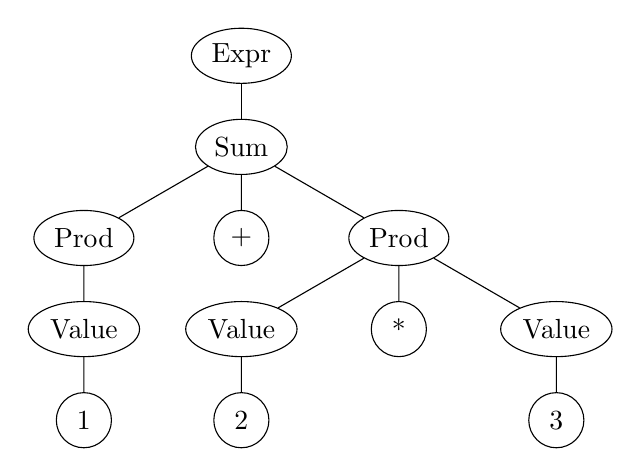
\begin{tikzpicture}[
      level distance=0.8cm,
      sibling distance=2cm,
      every node/.style={
         draw,
         shape=ellipse,
         minimum height=7mm,
         minimum width=7mm,
         inner sep=2pt,
         anchor=north
      }
   ]

      \node {Expr}
      child {node {Sum}
         child {node {Prod}
            child {node {Value}
               child {node {1}}
            }
         }
         child {node {+}}
         child {node {Prod}
            child {node {Value}
               child {node {2}}
            }
            child {node {*} }
            child {node {Value}
               child {node {3}}
            }
         }
      };
   \end{tikzpicture}
   
   \caption{Generated abstract syntax tree for the expression 1+2*3}
   \label{fig:generated-ast}
\end{figure*}


\section{Related work}

Atkinson and Griswold~\cite{atkinson2006-effective-pattern-matching} presents 
the matching tool TAWK, which extends extend the pattern syntax of AWK to 
support matching of abstract syntax trees. In TAWK, pattern syntax is 
language-independent, based on abstract tree patterns, and each pattern can 
have associated actions, which are written in C for generality, familirity 
and performance. Throughout the paper, a prototypical example of extracting 
a call-graph from a given code, giving examples in differents tools for 
pattern matching.
At a later section, we also present an extraction of a call-graph using the
tool developed in this paper.

Kopell et al.~\cite{kopell2018-language-parametric-transformation} presents an
approach for building source-to-source transformation that can run on multiple
programming languages, based on a representation called incremental parametric
syntax (IPS).
In IPS, languages are represented using a mixture of language-specific and 
generic parts. Transformations deal only with the generic fragments, but 
the implementer starts with a pre-existing normal syntax definition, and 
only does enough up-front work to redefine a small fraction of a language 
in terms of these generic fragments.
The IPS was implemented in a Haskell framework called \textit{Cubix}, 
and currentl supports C, Java, JavaScript, Lua, and Python.
They also demonstrate a whole-program refactoring for threading variables
through chains of function calls and three smaller source-to-source 
transformations, being a hoisting transformation, a test-coverage 
transformation and a the three-address code transformation.

Premtoon et al.~\cite{premtoon2020-code-search-equational-reasoning} presents 
a tool called \textit{Yogo}, that uses an approach to semantic code search 
based on equational reasoning, that considers not only the dataflow graph of 
a function, but also the dataflow graphs of all equivalents functions reachable 
via a set of rewrite rules. The tool is capable of recognizing differents 
variations of the same operation and also when code is an instance of a 
higher-level concept.
\textit{Yogo} is built on the \textit{Cubix} multi-language infraestructure and 
can find equivalent code in multiple languages from a single query.

Silva et al.~\cite{silva2021-refdiff} proposes \textit{RefDiff 2.0}, a 
multi-language refactoring detection tool. Their approach introduces a 
refactoring detection algorithm that relies on the Code Structure Tree 
(CST), a representation of the source code that abstract away the 
specificities of particular programming languages. 
The tool has results that are on par with state-of-the-art refactoring 
detection approaches specialized in the Java language and has support 
for two other popular programming languages: JavaScript and C,
demonstrating that the tool can be a viable alternative for multi-language
refactoring research and in practical applications of refactoring detection.

van Tonder and Le Goues~\cite{vanTonder2019-syntax-transformation-ppc} proposes
that the problem of automatically transforming programs can be decomposed such
that a common grammar expresses the central context-free language (CLF) 
properties shared by many contemporary languages and open extensions points
in the grammar allow customizing syntax and hooks in smaller parsers to handle
language-specific syntax, such as comments. The decomposition is made using a
Parser Parser combinator (PPC), a mechanism that generates parsers for matching
syntactic fragments in source code by parsing declarative user-supplied 
templates. 
This allows to detach from translating input programs to any particular 
abstract syntax tree representation, and lifts syntax rewriting to a 
modularly-defined parsing problem. 
They also evaluated \textit{Comby}, an implementation of the approach process 
using PPC, on a large scale multi-language rewriting across 12 languages, and 
validated effectiveness of the approach by producing correct and desirable 
lightweight transformations on popular real-world projects.

Matute et al.~\cite{matute2024-sequence-tree-matching} proposes a search
architecture that relies only on tokenizing a query, introducing a new 
language and matching algorithm to support tree-aware wildcards by building
on tree automata. They also present \textit{stsearch}, a syntactic search
tool leveraging their approach, which supports syntactic search even for
previously unparsable queries.

Ierusalimschy~\cite{ierusalimschy2009-lpeg} proposes the use of PEGs as a basis
for text pattern-mathing and presents LPEG, a pattern-matching tool based on 
PEGs for the Lua scripting language, and a Parsing Machine that allows a small 
and efficient implementation of PEGs for pattern matching. 
This allow LPEG to have both the expressive power of PEGs with the ease of use 
of regular expressions.
LPEG also seems specially suited for languages that are too complex for 
traditional pattern-matching tools but do not need a complex yacc-lex 
implementation, like domain-specific languages such as SQL and regular
expressions, and even XML.

\section{Conclusão}

Fazer um parágrafo finalizando a seção.

\cleardoublepage
  %\newpage\null\thispagestyle{empty}\newpage
  \chapter{Methodology}\label{chap:methodology}

This chapter presents the proposal of the pattern matching algorithm developed
during the work, as well as the  current state of its implementation.
Section~\ref{sec:parse-tress} details the semantics for producing a parse tree
from a parsing expression and their relation. Section~\ref{sec:patterns} presents 
the syntax and semantics for parse tree patterns, along with a typing (and subtyping)
relation. Section~\ref{sec:implementation-details} discusses some implementation
details. Finally, Section~\ref{sec:methodology-conclusion} concludes the chapter.

\section{Parse trees}\label{sec:parse-tress}

In order to proper define pattern matching over trees, we need
to define parse trees over an arbitrary PEG. We start by defining
tree syntax and a PEG semantics which produces, as a result, such
trees. Next, we present a typing relation which assigns a parsing
expression for a given tree. Such step is necessary to formally
state the equivalence between our proposed tree-producing semantics
and PEG original semantics proposed by Ford~\cite{ford2004-peg}.

Let \(G = (V, \Sigma, R, e_s)\) be an arbitrary PEG, the meta-variable \(a \in \Sigma\) an
arbitrary alphabet symbol, \(A \in V\) a variable and \(e\) a parsing expression.
The following context-free grammar defines the syntax of a parse tree:
\[
   \begin{array}{lcl}
      t & \to & \hat{\epsilon} \, \mid \, \hat{a} \, \mid \, A@t\,
                    \mid \, \langle t_1, t_2 \rangle\,
                    \mid \, L\:t \, \mid \, R\:t \, \mid \, [\,] \,\mid\,t \typecolon t\,
                    \mid \, \eta \\
   \end{array}
\]
Where \(\hat{\epsilon}\) represents that a parsing expression resulted in
success without consuming any symbol of its input, \(\hat{a}\) represents that
the parsing expression consumed the symbol \(a\) from the input, \(A@t\)
represents that the parsing of the rule \(A \leftarrow e \in R\) was succeesful
and $t$ is a tree for $e$. Notation
\(\langle t_1, t_2 \rangle\) represents that a sequence of parsing expressions
succeeded,
\(L \: t\) represents that the left branch in an ordered choice succeeded, while
\(R \: t\) represents that the right branch in an ordered choice succeeded.
\([]\) is an empty list of trees for $e$ and \(t_1  \typecolon  t_2\) denotes a list of
trees in which $t_1$ is a tree for $e$ and $t_2$ is a tree for $e^*$. Finally,
\(\eta\) represents that a not predicate was successful.

Executing a parsing expressions produces a parsing tree and is defined by an
inductively defined judgment that relates pairs formed by a parsing expression
and an input string to pairs formed by the produced tree and the remaining string.
Notation \((e,s_ps_r) \Downarrow_G (t,s_r)\) denote that parsing expression \(e\)
consumes the prefix \(s_p\) and produces the parse tree \(t\) from the input string
\(s_ps_r\) leaving the suffix \(s_r\). The notation \((e,s) \Downarrow_G \bot\)
denote the fact that \(s\) cannot be parsed by \(e\). We let meta-variable \(r\)
denote an arbitrary parsing result, i.e., either \(r\) is a pair \((t,s_r)\) or
\(\bot\). We say that an expression \(e\) fails if its execution over an input
produces \(\bot\); otherwise, it succeeds. Figure~\ref{fig:peg-tree-semantics}
defines the PEG semantics for production of a tree.

\begin{figure}[H]
   \[
      \begin{array}{cc}
         \infer[_{\{Eps\}}]{(\epsilon,s) \Downarrow_G (\hat{\epsilon},s)}{} &
         \infer[_{\{ChrS\}}]{(a,as_r) \Downarrow_G (\hat{a},s_r)}{} \\ \\
         \infer[_{\{ChrF\}}]{(a,bs_r) \Downarrow_G \bot}{a \neq b} &
         \infer[_{\{Var\}}]{(A,s) \Downarrow_G (A@t, r)}
                        {A \leftarrow e \in R & (e,s) \Downarrow_G (t,r)} \\ \\
         \multicolumn{2}{c}{
            \infer[_{\{Cat_{S1}\}}]{(e_1\,e_2,s_{p_1}s_{p_2}s_r) \Downarrow_G (\langle t_1,t_2 \rangle, s_r)}
                                 {(e_1,s_{p_1}s_{p_2}s_r) \Downarrow_G (t_1,s_{p_2}s_r) &
                                 (e_2,s_{p_2}s_r)\Downarrow_G (t_2,s_r)}
         } \\ \\
         \multicolumn{2}{c}{
            \infer[_{\{Cat_{F2}\}}]{(e_1\,e_2,s_ps_r) \Downarrow_G \bot}
                                 { (e_1,s_ps_r) \Downarrow_G (t_1,s_r) &
                                    (e_2,s_r) \Downarrow_G \bot}} \\ \\
         \infer[_{\{Cat_{F1}\}}]{(e_1\,e_2,s)\Downarrow_G \bot}{(e_1,s) \Downarrow_G \bot} &
         \infer[_{\{Alt_{S1}\}}]{(e_1\,/\,e_2,s_p\,s_r) \Downarrow_G (L \, t,s_r)}
                                {(e_1,s_p\,s_r)\Downarrow_G (t,s_r)} \\ \\
         \multicolumn{2}{c}{
            \infer[_{\{Alt_{S2}\}}]{(e_1\,/\,e_2,s_p\,s_r) \Downarrow_G R \, t}
                                  {(e_1,s_p\,s_r)\Downarrow_G \bot &
                                   (e_2,s_p\,s_r)\Downarrow_G t}
         } \\ \\
         \multicolumn{2}{c}{
            \infer[_{\{Star_{rec}\}}]{(e^\star,s_{p_1}s_{p_2}s_r) \Downarrow_G (t_1  \typecolon  t_2,s_r)}
                                 {(e,s_{p_1}s_{p_2}s_r) \Downarrow_G (t_1,s_{p_2}s_r) &
                                  (e^\star, s_{p_2}s_r) \Downarrow_G (t_2,s_r)}
         } \\ \\
         \infer[_{\{Star_{end}\}}]{(e^\star,s) \Downarrow_G ([\,],s)}
                                    {(e,s) \Downarrow_G \bot} &
         \infer[_{\{Not_F\}}]{(!\,e,s_p\,s_r) \Downarrow_G \bot}
                          {(e,s_p\,s_r) \Downarrow_G (t,s_r)}\\ \\
         \infer[_{\{Not_S\}}]{(!\,e,s) \Downarrow_G (\eta,s)}
         {(e,s) \Downarrow_G \bot}
           &
         \infer[_{\{ChrNil\}}]{(a,\epsilon) \Downarrow_G \bot}{}
      \end{array}
   \]
   \centering
   \caption{Parsing expressions operational semantics that produces a tree.}
   \label{fig:peg-tree-semantics}
\end{figure}

A parse tree is directly related to its underlying parsing expression.
We formalize this idea using a typing relation between grammars, trees and
parsing expressions. Notation $G\vdash t : e$ means that tree $t$ has
type $e$ using as assumption the variables and rules defined by grammar $G$.
Figure~\ref{fig:tree-typing} presents the rules of tree typing relation.

\begin{figure}[H]
  \[
    \begin{array}{cc}
      \infer[_{\{TEps\}}]{G \vdash \hat{\epsilon} : \epsilon}{} &
      \infer[_{\{TChr\}}]{G\vdash \hat{a} : a}{} \\ \\
      \infer[_{\{TVar\}}]{ G \vdash A@t : A}
                      {A \leftarrow e \in R(G) & G\vdash t : e} &
      \infer[_{\{TNot\}}]{G\vdash \eta :\: ! e}{}\\ \\
      \infer[_{\{TCat\}}]{G\vdash \langle t_1, t_2\rangle : e_1\,e_2}
                      {G\vdash  t_1 : e_1 & G\vdash t_2 : e_2} &
      \infer[_{\{TLeft\}}]{G\vdash L\:t : e_1 / e_2}
                       {G\vdash t : e_1} \\ \\
      \infer[_{\{TRight\}}]{G\vdash R\:t : e_1 / e_2}
                       {G\vdash t : e_2} &
      \infer[_{\{TNil\}}]{G \vdash [] : e^*}{}\\ \\
      \multicolumn{2}{c}{
        \infer[_{\{TCons\}}]{G \vdash t_1  \typecolon  t_2 : e^*}
                         {G\vdash t_1 : e &
                          G \vdash t_2 : e^*}
      }
    \end{array}
  \]
  \centering
  \caption{Typing relation for parse trees.}
  \label{fig:tree-typing}
\end{figure}

Rule \(_{TEps}\) means that the tree \(\hat{\epsilon}\) has type \(\epsilon\).
Rule \(_{TChr}\) means that the tree \(\hat{a}\) has type equal to the char consumed.
Rule \(_{TVar}\) specifies that a tree \(t\) has type \(A\) when there is a rule 
\(A \leftarrow e\) in the set of rules from grammar \(G\) and \(t\) is produced
by \(e\). Rule \(_{TNot}\) means that tree \(\eta\) has type \(!e\) for all \(e\). 
Rule \(_{TCat}\) specifies that a tree \(\langle t_1, t_2\rangle\) has type 
\(e_1\:e_2\) if \(t_1\) and \(t_2\) have types \(e_1\) and \(e_2\), respectively. 
Rules \(_{TLeft}\) and \(_{TRight}\) says that a tree \(t\) has type \(e_1 / e_2\) 
if t has type \(e_1\) or t has type \(e_2\). Rules \(_{TNil}\) means that tree 
\([]\) has type \(e^\star\) for all \(e\) and \(t_1  \typecolon  t_2\) has type \(e^\star\) 
if \(t_1\) has type \(e\) and \(t_2\) has type \(e^\star\).
 
Next, we need to show that our tree producing semantics is equivalent to
the original semantics for PEGs. Intuitively, our trees are a strutured
representation of the prefix parsed by a grammar. We name the textual
representation of a parse tree as its flattening which is defined
by recursion on the structure of the parse tree (Figure~\ref{fig:flattening-tree}).

\begin{figure}[H]
  \[
    \begin{array}{lcl}
      |\hat{\epsilon}| & = & \epsilon\\
      |\hat{a}| & = & a\\
      |A@t| & = & |t|\\
      |\langle t_1, t_2 \rangle| & = & |t_1|\,|t_2|\\
      |L\:t| & = & |t|\\
      |R\:t| & = & |t|\\
      |[]| & = & \epsilon \\
      |t_1  \typecolon  t_2| & = & |t_1|\,|t_2|\\
    \end{array}
  \]
  \centering
  \caption{Flattening of a parse tree.}
  \label{fig:flattening-tree}
\end{figure}

Flattening a parse tree essentially means to collapse the tree's structure into a 
a string, containing the characters at the tree's leaves. \(\hat{\epsilon}\) and
\([]\) both flattens to empty string \(\epsilon\) and \(\hat{a}\) flattens to 
symbol \(a\), while \(A@t\) flattens \(t\). Flattening both \(\langle t_1, t_2 
\rangle\) and \(t_1  \typecolon  t_2\) means concatening the flatenning of \(t_1\) 
and of \(t_2\), while flattening \(L\:t\) and \(R\:t\) just flattens \(t\) directly. 

The typing relation specifies what kind of parse trees are possible to be
constructed for a given parsing expression. Using the flatenning function,
we can formally describe the relation between our tree producing semantics
and PEG original semantics.
The next theorem presents this result.

\begin{theorem}[Semantics equivalence]
  Let $G$ be an arbitrary PEG. If $G \vdash t : e$ then $(e, |t|) \Downarrow_G (t, \epsilon)$ and
  $(e, |t|)\Rightarrow_G (|t|, \epsilon)$
\end{theorem}
\begin{proof}
  Induction over the derivation of $G \vdash t : e$ using the correspondent semantics rule in each case.
\end{proof}

In the next section, we use parse trees and its semantics to formally define
a pattern matching algorithm.

\section{Parse tree patterns and its semantics}\label{sec:patterns}

We start this section presenting pattern syntax and its typing relation.
Next, we present a subtyping relation between parsing expression which allow us
to describe coercions between patterns to allow both an easy specification of tree
patterns and immediate implementation of pattern matching for trees.

\subsection{Pattern syntax and typing relation}

In simple terms, patterns describe the user intendeed structure for a given
input parse tree. Pattern syntax shares the same structure of tree syntax with
the addition of \emph{pattern-variables}, which will match any tree of a given type.
The syntax of pattern is presented next.

\[
    \begin{array}{lcl}
        p & \to & \epsilon \, \mid \, a \, \mid \, A@p\, \mid \,p_1\:p_2\,
                \mid\,p_1\,/\,p_2\, \mid \,p^\star\, \mid \,!\,p
                \mid \, M : e
    \end{array}
\]
Where \(\epsilon\) is a pattern that matches with the tree of
empty string (\(\hat{\epsilon}\)),
\(a\) matches only with the tree of the symbol \(a\) (\(\hat{a}\)), \(A@p\) matches
with a subtree of type \(e\) and \((A, e) \in R\), \(p_1\:p_2\) matches if both
\(p_1\) and \(p_2\) matches sequentially. \(p_1\,/\,p_2\) matches if one of \(p_1\)
or \(p_2\) matches, \(p^\star\) will try to match \(p\) sequentially as many times
as possible, \(!p\) matches only if \(p\) does not matches. \(M : e\) is a pattern
variable that matches with any tree \(t : e\).

Since patterns are similar to trees, we also define a typing relation for patterns.

\begin{figure}[H]
  \[
    \begin{array}{cc}
      \infer[_{\{PEps\}}]{G \vdash \epsilon : \epsilon}{} &
      \infer[_{\{PChr\}}]{G\vdash a : a}{} \\ \\
      \infer[_{\{PVar\}}]{ G \vdash A@p : A}
                      {A \leftarrow e \in R(G) & G\vdash p : e} &
      \infer[_{\{PNot\}}]{G\vdash !p: ! e}{G\vdash p : e}\\ \\
      \infer[_{\{PCat\}}]{G\vdash p_1, p_2 : e_1\,e_2}
                      {G\vdash  p_1 : e_1 & G\vdash p_2 : e_2} &
      \infer[_{\{PLeft\}}]{G\vdash p_1 : e_1 / e_2}
                       {G\vdash p_1 : e_1} \\ \\
      \infer[_{\{PRight\}}]{G\vdash p_2 : e_1 / e_2}
                       {G\vdash p_2 : e_2} &
      \infer[_{\{PStar\}}]{G \vdash  p^ * : e^*}{G \vdash p : e}\\ \\
   \end{array}
  \]
  \centering
  \caption{Typing relation for patterns.}
  \label{fig:pattern-typing}
\end{figure}

% \subsection{Subtyping for and for patterns}
\subsection{Subtyping for parsing expressions and patterns}

When specifying patterns over choice expressions, we may want to match against 
a specific branch of a choice. Instead of specifying a choice pattern that will 
fail for all other branches besides the intended one, we would like to specify 
one single pattern that would match only with the intended branch, decreasing 
the size of the written pattern. 
Consider the PEG shown in Figure~\ref{fig:peg-arith-expressions}. If we want to, 
e.g., match a multiplication between a parenthesized expressions and a number, 
we would have to write two choice patterns for rule F: one that accepts a number, 
but reject a parenthesized expression (e.g. \(V_1:n / \bot_E\)) and one the rejects 
a number, but accepts a parenthesized expression (e.g. \(\bot_n / '(' V_2:E ')'\)).
Instead, it would be easir to just specify the patterns that matches against numbers
(\(V_1:n\)) and against parenthesized expressions (\(V_2:E\)) and let the algorithm
fill the missing part.
To do this, we introduce a subtyping relation and subtype-based coercion both 
for parsing expressions and patterns.

We let notation $e <: e'$ denote that expression $e$ is a subtype of expression $e'$.
The idea of the subtyping relation is to express that is possible to ``coerce'' a
tree $t$, such that $G \vdash t : e$,  to a tree $t'$, such that $G \vdash t' : e'$,
in a way that the coercion preserves the parsed string, i.e., $|t| = |t'|$.
Since patterns shares all the structure of parse trees, the coercion reasoning
applies to patterns. The main objective of this section is to define, in a precise
manner, the subtype-based coercion for patterns.

We start by defining the subtype relation between parsing expressions.

\begin{figure*}[ht]
    \[
        \begin{array}{cccc}
            \infer[_{\{Refl\}}]{e <: e}{} &
            \infer[_{\{Alt_{Left}\}}]{e_1 <: e_2 / e_3}{e_1 <: e_2} &
            \infer[_{\{Alt_{Right}\}}]{e_1 <: e_2 / e_3}{e_1 <: e_3} &
            \infer[_{\{Star\}}]{e_1^n <: e_2^\star}{n \geq 0 & e_1 <: e_2}
        \end{array}
    \]
    \centering
    \caption{Subtype relation for parsing expressions}
    \label{fig:subtype-relation}
\end{figure*}

The first rule denote a common requirement for subtyping: it is
a reflexive relation. Next, we have two rules for dealing
with the choice operator. The first shows that the left component of a choice
is a subtype of $e_1/e_2$. The same holds for the right operand of ordered choice
expression. Finally, we have that $e_1^n$ is a subtype of $e_2^\star$, whenever
$e_1 <: e_2$. Notation $e^n$ denotes the repeated concatenation of $e$, as usual.

Next, we define the syntax of terms to denote subtyping proofs, as follows:

\[
  \begin{array}{lcl}
    d & \to & \mathbf{refl}
      \: \mid \: \mathbf{Inl}\,d
      \: \mid \: \mathbf{Inr}\,d
      \: \mid \: \mathbf{Rec}\,d
  \end{array}
\]
Term $\mathbf{refl}$ denotes a proof for $e<:e$ and $\mathbf{Inl}\:d$ denotes
a subtyping derivation for $e_1 <:e_2 / e_3$, where $d$ represents the
subderivation for $e_1 <: e_2$. Same reasoning applies to $\mathbf{Inr}$ and
$\mathbf{Rec}$ for deductions of $e_1 <: e_2 / e_3$ and $e_1^n <: e_2^*$,
respectively.

Finally, we show that the subtyping relation for parsing expressions is
decidable.

\begin{theorem}[Decidability of subtyping]
  For any parsing expressions $e_1$ and $e_2$, we have that either $e_1 <: e_2$ or
  that $\neg (e_1 <: e_2)$
\end{theorem}
\begin{proof}
  Induction over the structure of $e_1$ and case analysis over the structure of $e_2$
  using the definition of the subtyping relation.
\end{proof}


\subsection{Subtype-based coercion for patterns}

In this section we define an algorithm for coercing patterns using the subtyping
relation between parsing expressions. The algorithm is defined by equations over
pattern trees and subtyping terms.

\[
  \begin{array}{lcl}
    \mathbf{coerce}(p,\mathbf{refl}) & = & p\\
    \mathbf{coerce}(p,\mathbf{Inl}\:d) & = & \mathbf{coerce}(p,d)\,/\,\bot_p\\
    \mathbf{coerce}(p,\mathbf{Inr}\:d) & = & \bot_p\,/\,\mathbf{coerce}(p,d)\\
    \mathbf{coerce}(p^n,\mathbf{Rec}\:d) & = & \mathbf{coerce}(p,d)^\star\\
  \end{array}
\]

Notation $\bot_p$ denotes the patterns which fails for any parse tree and it is 
equivalent to pattern \(!M : e\), where \(p : e\). Intuitively, the coercion allow 
us to match trees for the choice or star operator by just specifying the desired 
component, for ordered choice, or a specific number of matchings for the star 
operator. The coerce function satisfies the following property.

\begin{theorem}[Correctness of coerce]\label{thm:coerce-correct}
  Let $G = (V,\Sigma, R, e_s)$ be an arbitrary PEG, $p$ a pattern such that
  $G\vdash p : e$ and that $d$ is a proof term for $e <: e'$, for some
  $e'$. Then, $G\vdash \mathbf{coerce}(p,d) : e'$.
\end{theorem}
\begin{proof}
  Induction over the structure of $G\vdash p : e$ and case analysis over
  the derivation of $e <: e'$ using the definitions of $\mathbf{coerce}$ and
  the typing relation for patterns.
\end{proof}

Now with the definition of subtyping-based coercion for patterns we are
ready to formally define an algorithm for pattern matching parse trees.

\subsection{A semantics for parse trees pattern matching}

Before presenting the semantics for pattern matching we need some additional
definitions. We name a \emph{match} a sequence between pattern variables
and parse trees. We let meta-variable $S$ to represent an arbitrary match.
In simple terms, the result of matching a pattern against a tree is a sequence
which holds the trees associated with each pattern variable matched.
Notation $[M \mapsto t]$ denotes the singleton match between
a pattern-variable $M$ with a tree $t$, $\bullet$ denotes an empty match and
$\uplus$ denotes sequence concatenation. We let meta-variable $r$
denote either a match $S$ or a failure, $\bot$.

Matching a pattern $p$ against a tree $t$ is a process defined by an inductively
defined judgment $G \vdash p : e; t \leadsto S$, where $G$ denotes a PEG,
$p$ a pattern for $e$, $t$ a parse tree and $S$ is the result match.
The algorithm is presented in Figure~\ref{fig:pattern-semantics}.

\begin{figure}[H]
  \[
    \begin{array}{cc}
      \infer[_{\{PPVar\}}]{G\vdash M_1 : e ; t_1 \leadsto [M_1 \mapsto t_1]}{G \vdash t_1 : e} &
      \infer[_{\{PEps\}}]{G \vdash \epsilon : \epsilon ; \hat{\epsilon} \leadsto \bullet}{} \\ \\
      \infer[_{\{PChr\}}]{G\vdash a : a ; \hat{a} \leadsto \bullet}{} &
      \infer[_{\{PChrf\}}]{G \vdash a : a  ; \hat{b} \leadsto \bot}{a \neq b}\\ \\
        \infer[_{\{PVar\}}]{G\vdash A@p : A ; A@t \leadsto r}
                        {\begin{array}{c}
                           A \leftarrow e \in R(G) \\
                           G\vdash p : e ; t \leadsto r
                         \end{array}}
        &
        \infer[_{\{PCat\}}]{G\vdash p_1\,p_2 : e_1\,e_2; \langle t_1, t_2 \rangle \leadsto S_1 \uplus S_2}
                        {\begin{array}{c}
                           G\vdash p_1 :e_1 ; t_1 : \leadsto S_1 \\
                           G\vdash p_2 :e_2 ; t_2 :\leadsto S_2
                        \end{array}}\\ \\
      \infer[_{\{PCat1\}}]{G\vdash p_1\,p_2 : e_1 \, e_2  ; \langle t_1, t_2 \rangle \leadsto \bot}
                      {G\vdash p_1 : e_1 ; t_1 \leadsto \bot} &
      \infer[_{\{PCat2\}}]{G\vdash p_1\,p_2 :e_1\,e_2 ; \langle t_1, t_2 \rangle \leadsto \bot}
                        {\begin{array}{c}
                            G\vdash p_1 :e_1 ; t_1 \leadsto S_1 \\
                            G\vdash p_2 :e_2 ; t_2\leadsto \bot
                         \end{array}} \\ \\
      \infer[_{\{PLeft\}}]{G \vdash p_1\,/\,p_2 ;: e_1\,/\,e_2\ ;L\:t \leadsto r}
                       {G\vdash p_1 :e_1 ; t\leadsto r} &
      \infer[_{\{PRight\}}]{G \vdash p_1\,/\,p_2 : e_1\,/\,e_2; R\:t \leadsto r}
                       {G\vdash p_2 : e_2; t \leadsto r} \\ \\
      \infer[_{\{PNot\}}]{G \vdash !\,p : ! e ; \eta \leadsto \bullet}
                      {G \vdash p : e ; t \leadsto \bot} &
      \infer[_{\{PNot1\}}]{G \vdash !\,p : ! e ; \eta \leadsto \bot}
                       {G \vdash p : e ; \eta \leadsto S}\\ \\

      \infer[_{\{PStarn\}}]{G \vdash p^\star : e^\star ; [] \leadsto \bullet}{} &
      \infer[_{\{PStarf\}}]{G\vdash p^\star : e^\star ; t_1  \typecolon  t_2 \leadsto S_1 \uplus S_2}
                        {\begin{array}{c}
                           G \vdash p : e ; t_1 \leadsto S_1\\
                           G \vdash p^\star : e^\star ; t_2 \leadsto S_2
                         \end{array}}\\ \\
    \end{array}
  \]
  \centering
  \caption{Semantics for pattern matching parse trees.}
  \label{fig:pattern-semantics}
\end{figure}

Rule \(_{PPVar}\) specifies that a pattern variable \(M : e\) matches with any
tree \(t\) of type \(e\) and binds \(t\) to \(M\). Rule \(_{PEps}\) specifies 
that the pattern \(\epsilon\) matches only with with tree \(\hat{\epsilon}\),
but does not bind anything. Rules \(_{PChr}\) and \(_{PChrf}\) says that 
a pattern of type \(a\) matches only with the tree \(\hat{a}\) and fails if 
matched against any other symbol. Rule \(_{PVar}\) specifies that pattern \(A@p\)
matches only if there is a rule \(A \leftarrow e \in R(G)\) and \(p\) has type \(e\).
Rules \(_{PCat1}\) and \(_{PCat2}\) says that if either \(p_1\) or \(p_2\) in
sequence \(p_1\:p_2\) does not match, then the whole sequence does not match either.
Otherwise, rule \(_{PCat}\) specifies that the the resulting binds are concatenated.
The rules for choice \(_{PLeft}\) and \(_{PRight}\) specifies that the left branch 
of a pattern matches only with a tree \(L\:t\) and the right branch matches only
with a tree \(R\:t\). Rules for the negation predicate \(_{PNot}\) and \(_{PNot1}\)
says that \(!p\) matches with \(\eta\) only if pattern \(p\) fails to match 
and it does not generate any binds, otherwise \(!p\) fails.
Rule \(_{PStarn}\) specifies that pattern \(p^\star\) always matches against \([]\),
but does not bind anything and rule \(_{Pstarf}\) says that \(p^\star\) matches 
with \(t_1 \typecolon t_2\) if \(p\) matches with \(t_1\) and \(p^\star\) matches 
with \(t_2\), i.e. it tries to match \(p\) with every tree in the list, and 
concatenates all the resulting binds in each match.

\begin{example}
  Consider the PEG for arithmetic expressions shown in Figure~\ref{fig:peg-arith-expressions}, 
  the string \((1+2)*3\) and the pattern \((\text{X}:E)*\text{Y}:F\), where X 
  and Y are pattern variables of type \(E\) and \(F\), respectively. 
  Some things to note on the pattern are: 
  1) The pattern \((\text{X}:E)\) has type \(F\), \((\text{X}:E):F\), since it 
  matches with the right branch of the choice expression of rule 
  \(F \leftarrow \text{n / '(' E ')'}\), by rule \(_{PRight}\); and
  2) The pattern \(* \text{Y}:F\) has type \((* \text{Y}:F)^\star\), by rule 
  \(_{PStar}\) where \(n = 1\), and matches without problems.
  Since all components of the pattern are valid, then the whole pattern 
  \((\text{X}:E)*\text{Y}:F\) is also valid and has type \(T\),
  \(\{(\text{X}:E)*\text{Y}:F\}:T\).

  By the concatenation rule, the opening parenthesis (`(') matches, the pattern 
  variable X binds to expression \(1+2\), the closing parenthesis (`)') and 
  multiplication operator (`*') also matches and finally pattern variable Y 
  binds to \(3\).
  The matches found are \([X \mapsto 1+2, Y \mapsto 3]\).
\end{example}

Given a match $S$ and a pattern $p$, we denote by $S[p]$ the parse tree
obtained by replacing pattern variables in p by its corresponding tree
in $S$. Now, we state the main property of the matching algorithm.

\begin{theorem}[Matching correctness]\label{thm:matching-correct}
  Let $G = (V,\Sigma,R, e_s)$ be an arbitrary PEG, $p$ a pattern,
  $e$ a parsing expression and $t$ a parse tree. If $G \vdash p : e$, $G \vdash t : e$ and
  $G\vdash p : e ; t \leadsto S$ then $S[p] = t$.
\end{theorem}
\begin{proof}
  By induction over the structure of derivation of $G\vdash p : e ; t \leadsto S$.
\end{proof}

While previous theorem result is important, it is limited: it only applies to
trees and patterns that have same parsing expression type $e$. Thanks to coercion,
we can use the algorithm whenever the pattern and tree types does satisfy the
subtyping relation.

\begin{corollary}
Let $G = (V,\Sigma,R, e_s)$ be an arbitrary PEG, $p$ a pattern,
$e$ a parsing expression and $t$ a parse tree. If $G \vdash p : e$, $G \vdash t : e'$,
  $d :: e <: e'$ and $G\vdash \mathbf{coerce}(p,d) : e' ; t \leadsto S$ then $S[p] = t$.
\end{corollary}
\begin{proof}
  Immediate from theorems~\ref{thm:matching-correct} and~\ref{thm:coerce-correct}.
\end{proof}

\section{Implementation details}\label{sec:implementation-details}

This section presents implementation details and the tool architecture. 
Figure~\ref{fig:tool-diagram} presents a diagram of the tool structure.

\begin{figure*}
  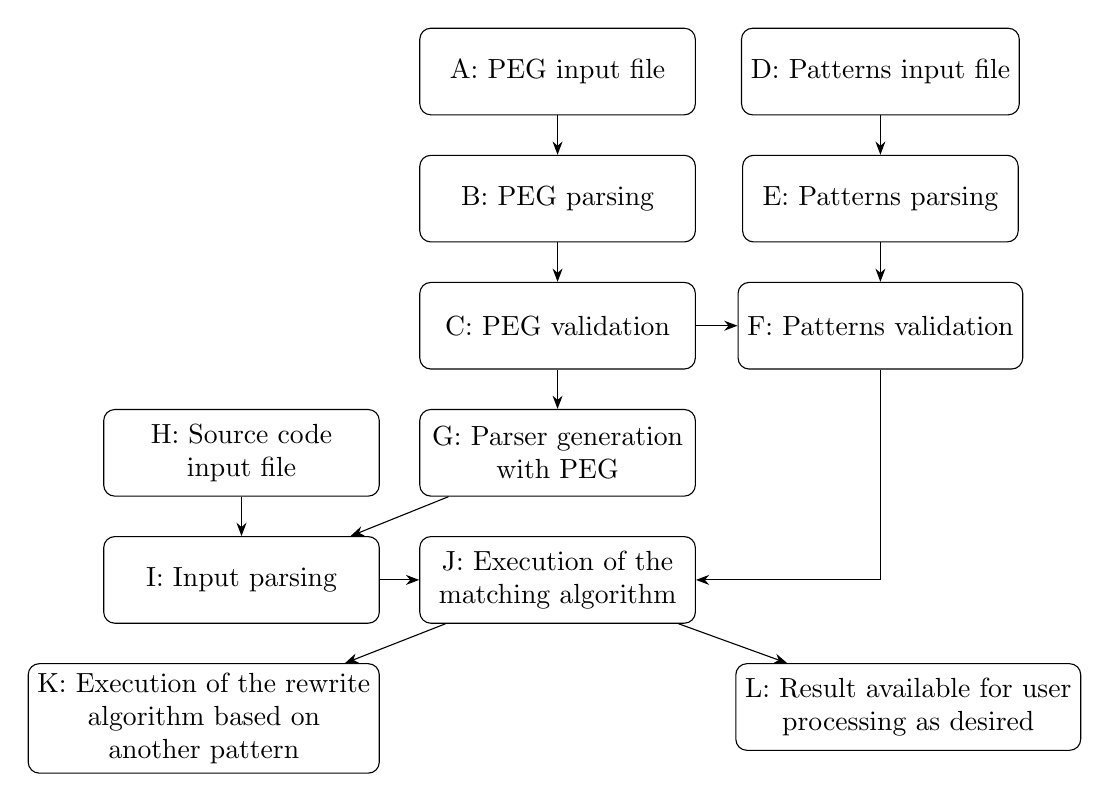
\begin{tikzpicture}[
      node distance=0.5cm and 0.5cm,
      every node/.style={draw, align=center, rounded corners, minimum width=3.5cm, minimum height=1.1cm},
      ->, >=Stealth
    ]
  
    \node (A) at (0,0) {A: PEG input file};
    \node (D) at (4.1,0) {D: Patterns input file};
  
    \node[below=of A] (B) {B: PEG parsing};
    \node[below=of D] (E) {E: Patterns parsing};
  
    \node[below=of B] (C) {C: PEG validation};
    \node[below=of E] (F) {F: Patterns validation};
  
    \node[below=of C] (G) {G: Parser generation\\with PEG};
    \node[left=of G] (H) {H: Source code\\input file};
  
    \node[below=of H] (I) {I: Input parsing};
    \node[below=of G] (J) {J: Execution of the\\matching algorithm};
  
    \node[below left=0.5cm and 0.5cm of J] (K) {
      K: Execution of the rewrite\\algorithm based on\\another pattern
    };
    \node[below right=0.5cm and 0.5cm of J] (L) {
      L: Result available for user\\processing as desired
    };
  
    \draw (A) -- (B);
    \draw (B) -- (C);
    \draw (C) -- (G);
    \draw (D) -- (E);
    \draw (E) -- (F);
  
    \draw (C) -- (F);
  
    \draw (H) -- (I);
  
    \draw (G) -- (I);
    \draw (I) -- (J);
  
    \draw (F) |- (J);  % faz a curva
  
    \draw (J) -- (K);
    \draw (J) -- (L);
  
  \end{tikzpicture}
  \centering
  \caption{Tool diagram}
  \label{fig:tool-diagram}
\end{figure*}

We define two new operators for PEGs: flatten \((^\wedge e)\) and indentation
\((e_1 > e_2)\). The former flattens the parsed tree in one single node that turns
into a terminal (and can be matched as such via patterns) and the latter, acts as 
the sequence \(e_1\:{e_2}^\star\) with the restriction that \({e_2}^\star\) must 
be indented with respect to \(e_1\) and matches as if it was a normal sequence.

While parsing a PEG (Node B), a sequence (e.g. \(e_1\:e_2\:e_2\)) of expression 
is always nested to the right (\(e_1\:(e_2\:e_3)\)) and operators \(\&\), \(?\) 
and \(+\) have specific behaviour: \(\&e\) generates the equivalent expression 
\(!!e\), \(e?\) generates \(e / \epsilon\) and \(e^+\) generates \(e \: e^\star\).
After parsing a PEG, we check if the PEG is valid (Node C), checking if it does 
not have left recursion or a parsing expression that accepts the empty string 
inside a star (\(^\star\)), since it may cause the PEG to loop indefinitely.

Pattern validation includes replacing references to other patterns with the
pattern itself, coercing the patterns if necessary and checking if the pattern 
follows the input PEG's structure. If any pattern makes reference to an undefined
pattern, the algorithm returns an error. To make the replacement between patterns, 
we create a dependency graph between the patterns, topologically sort and replace 
the references so that no resulting pattern contains references to other patterns 
and can be treated as a single pattern. This is done so that it is possible to write 
the patterns in any order, but no set of patterns may have circular dependency.

\section{Conclusion}\label{sec:methodology-conclusion}

This chapter presented the formalization for producing parse trees from an arbitrary
PEG, the formalization for parse trees patterns and the matching semantics, and 
a subtyping relation between parsing expression that applies both to the parse 
trees and the patterns. Finally, current implementation details were presented,
detailing specific behaviour for some operators and some validations done to 
ensure the PEG and patterns can be executed safely.

\cleardoublepage

  % \cleardoublepage
  \chapter{Results}\label{chap:results}



\cleardoublepage
  % \cleardoublepage
  \chapter{Schedule and Expected results}\label{chap:future-work}

This chapter presents the next steps for the development of this work and 
estimated deadlines. They are not precise and can change depending on the results
obtained. The remaining activities are enumerated below.

\begin{enumerate}
    \item Correct and terminate the pattern matching algorithm based on the 
        presented formalization.
    \item Testing and proofs of properties on patterns.
    \item Submission of a paper.
    \item Writing and presentation.
\end{enumerate}

The intended continuation of this is work is summarized on Table~\ref{table:schedule}.

\begin{table}[ht]
    \centering
    \caption{Intended schedule of future work}
    \label{table:schedule}
    \begin{tabular}{ll}
        \hline
        \textbf{Task} & \textbf{Deadline} \\
        \hline
        --- & ---\\
        \hline
    \end{tabular}
\end{table}
  % \cleardoublepage
  % \chapter{Conclusion}\label{chap:conclusion}



\cleardoublepage


  \backmatter
  \bibliographystyle{coppe-unsrt}
  \bibliography{thesis}

  \appendix
  \chapter{Simplified Python PEG}\label{append:python-peg}

% \[
% \begin{array}{ll}
%     \mathtt{file}           & \leftarrow \mathtt{(blank* \, newline)* \, statement+} \\
%     \mathtt{statement}      & \leftarrow \mathtt{(compound / simple / comment) \, blank* \, newline*} \\
%     \mathtt{compound}       & \leftarrow \mathtt{function\_def / if\_stmt / while\_stmt / for\_stmt} \\
%     \mathtt{function\_def}  & \leftarrow \mathtt{("def" \, space \, identifier \, "(" \, space \, id\_list? \, ")" \, space \, ":") > statement} \\
%     \mathtt{if\_stmt}       & \leftarrow \mathtt{(("if" \, space \, expression \, ":") > statement) (elif\_block / else\_block)?} \\
%     \mathtt{elif\_block}    & \leftarrow \mathtt{(("elif" \, space \, expression \, ":") > statement) (elif\_block / else\_block)?} \\
%     \mathtt{else\_block}    & \leftarrow \mathtt{("else" \, space \, ":") > statement} \\
%     \mathtt{while\_stmt}    & \leftarrow \mathtt{("while" \, space \, expression \, ":") > statement} \\
%     \mathtt{for\_stmt}      & \leftarrow \mathtt{("for" \, space \, identifier \, space \, "in" \, space \, expression \, ":") > statement} \\
%     \mathtt{simple}         & \leftarrow \mathtt{import\_stmt / assignment / return\_stmt / expression} \\
%     \mathtt{return\_stmt}   & \leftarrow \mathtt{"return" \, space \, expr\_list} \\
%     \mathtt{import\_stmt}   & \leftarrow \mathtt{simple\_import / from\_import} \\
%     \mathtt{simple\_import} & \leftarrow \mathtt{"import" \, space \, identifier} \\
%     \mathtt{from\_import}   & \leftarrow \mathtt{"from" \, space \, identifier \, space \, "import" \, space (id\_list / "*")} \\
%     \mathtt{assignment}     & \leftarrow \mathtt{id\_list \, space \, attr \, space \, expression} \\
%     \mathtt{attr}           & \leftarrow \mathtt{"=" / "+=" / "-=" / "*=" / "/="} \\
%     \mathtt{expression}     & \leftarrow \mathtt{or\_expr ("or" \, space \, or\_expr)*} \\
%     \mathtt{or\_expr}       & \leftarrow \mathtt{and\_expr ("and" \, space \, and\_expr)*} \\
%     \mathtt{and\_expr}      & \leftarrow \mathtt{"not" \, space \, comparison / comparison} \\
%     \mathtt{comparison}     & \leftarrow \mathtt{sum (op\_comp \, sum)*} \\
%     \mathtt{sum}            & \leftarrow \mathtt{term (op\_term \, term)* } \\
%     \mathtt{term}           & \leftarrow \mathtt{factor (op\_factor \, factor)*} \\
%     \mathtt{factor}         & \leftarrow \mathtt{power (op\_power \, power)*} \\
%     \mathtt{power}          & \leftarrow \mathtt{"-" \, neg / neg} \\
%     \mathtt{neg}            & \leftarrow \mathtt{primary \, space / "(" \, space \, expression \, ")" \, space} \\
%     \mathtt{op\_comp}       & \leftarrow \mathtt{("==" / "!=" / "<=" / ">=" / "<" / ">") \, space} \\
%     \mathtt{op\_term}       & \leftarrow \mathtt{("+" / "-") \, space} \\
%     \mathtt{op\_factor}     & \leftarrow \mathtt{("*" / "/" / "\%") \, space} \\
%     \mathtt{op\_power}      & \leftarrow \mathtt{"**" \, space} \\
%     \mathtt{primary}        & \leftarrow \mathtt{function\_call / array\_access / "[" \, items? \, "]" / atom} \\
%     \mathtt{function\_call} & \leftarrow \mathtt{identifier \, space \, "(" \, space \, expr\_list? \, ")" ("." \, primary)?} \\
%     \mathtt{array\_access}  & \leftarrow \mathtt{identifier \, space \, "[" \, space \, expression \, "]" ("." \, primary)?} \\
%     \mathtt{atom}           & \leftarrow \mathtt{"True" / "False" / "None" / number / strings / identifier} \\
%     \mathtt{expr\_list}     & \leftarrow \mathtt{expr1 \, space (sep \, expr1 \, space)*} \\
%     \mathtt{expr1}          & \leftarrow \mathtt{(single\_id \, space \, "=" \, space)? \, expression} \\
%     \mathtt{items}          & \leftarrow \mathtt{expression (sep \, expression \, space)*} \\
%     \mathtt{id\_list}       & \leftarrow \mathtt{identifier \, space (sep \, identifier \, space)*} \\
%     \mathtt{sep}            & \leftarrow \mathtt{"," \, space} \\
%     \mathtt{^strings}       & \leftarrow \mathtt{fstring / string} \\
%     \mathtt{fstring}        & \leftarrow \mathtt{"f" \, string} \\
%     \mathtt{string}         & \leftarrow \mathtt{['] (!['] char)* ['] / ["] (!["] char)* ["]} \\
%     \mathtt{char}           & \leftarrow \mathtt{[a-zA-Z0-9 :{}.,;^+-*/\%()\_!?\text{áéúçã}] / "[" / "]"} \\
%     \mathtt{^identifier}    & \leftarrow \mathtt{single\_id ("." \, single\_id)*} \\
%     \mathtt{single\_id}     & \leftarrow \mathtt{[a-zA-Z] [a-zA-Z0-9\_]*} \\
%     \mathtt{^number}        & \leftarrow \mathtt{[0-9]+} \\
%     \mathtt{space}          & \leftarrow \mathtt{" \, "*} \\
%     \mathtt{^blank}         & \leftarrow \mathtt{comment / " \, "} \\
%     \mathtt{^newline}       & \leftarrow \mathtt{"\backslash r\backslash n" / "\backslash r" / "\backslash n"} \\
% \end{array}
% \]

\begin{verbatim}
file          <- (blank* newline)* statement+
statement     <- (compound / simple / comment) blank* newline*
compound      <- function_def / if_stmt / while_stmt / for_stmt
function_def  <- ("def" space identifier "(" space id_list? ")" space 
                 ":") > statement
if_stmt       <- (("if" space expression ":") > statement) 
                 (elif_block / else_block)?
elif_block    <- (("elif" space expression ":") > statement) 
                 (elif_block / else_block)?
else_block    <- ("else" space ":") > statement
while_stmt    <- ("while" space expression ":") > statement
for_stmt      <- ("for" space identifier space "in" space expression 
                 ":") > statement
simple        <- import_stmt / assignment / return_stmt / expression
return_stmt   <- "return" space expr_list
import_stmt   <- simple_import / from_import
simple_import <- "import" space identifier
from_import   <- "from" space identifier space "import" space 
                 (id_list / "*")
assignment    <- id_list space attr space expression
attr          <- "=" / "+=" / "-=" / "*=" / "/="
expression    <- or_expr ("or" space or_expr)*
or_expr       <- and_expr ("and" space and_expr)*
and_expr      <- "not" space comparison / comparison
comparison    <- sum (op_comp sum)*
sum           <- term (op_term term)* 
term          <- factor (op_factor factor)*
factor        <- power (op_power power)*
power         <- "-" neg / neg
neg           <- primary space / "(" space expression ")" space
op_comp       <- ("==" / "!=" / "<=" / ">=" / "<" / ">") space
op_term       <- ("+" / "-") space
op_factor     <- ("*" / "/" / "%") space
op_power      <- "**" space
primary       <- function_call / array_access / "[" items? "]" 
                 / atom
function_call <- identifier space "(" space expr_list? ")" 
                 ("." primary)?
array_access  <- identifier space "[" space expression "]" 
                 ("." primary)?
atom          <- "True" / "False" / "None" / number / strings 
                 / identifier
expr_list     <- expr1 space (sep expr1 space)*
expr1         <- (single_id space "=" space)? expression
items         <- expression (sep expression space)*
id_list       <- identifier space (sep identifier space)*
sep           <- "," space
^strings      <- fstring / string
fstring       <- "f" string
string        <- ['] (!['] char)* ['] / ["] (!["] char)* ["]
char          <- [a-zA-Z0-9 :{}.,;^+-*/%()_!?áéúçã] / "[" / "]"
^identifier   <- single_id ("." single_id)*
single_id     <- [a-zA-Z] [a-zA-Z0-9_]*
^number       <- [0-9]+
space         <- " "*
^blank        <- comment / " "
^comment      <- "#" char*
^newline      <- "\r\n" / "\r" / "\n"
\end{verbatim}
\end{document}
